\chapter{Plataforma PyBoKids 2.0}
\label{cap:PyBoKids}
En este capítulo explicaremos el proceso seguido para desarrollar las bibliotecas Arduino y Python (ver en \cite{arduinolenguaje}, \cite{PythonRef}), explicando el código y las distintas necesidades que han surgido durante el desarrollo. \\
Como se explicó en el Capítulo \ref{cap:infra}, se ha utilizado Arduino  y su IDE nativo para esta programación, y Python 3 y un editor de texto estándar (en este caso, Visual Studio Code, de Microsoft) para la programación en Python. 

\section{Diseño}\label{sec:diseño}
Lo primero en el diseño de la plataforma ha sido el modelo ''PC - Residente''. Partiendo de la premisa dada de programación del robot en Python, era necesaria una forma para que, dado que la placa base funciona en Arduino, la comunicación Serial\footnote{Comunicación secuencial de información a través de un canal, electrónico en este caso} funcionara entre los dos lenguajes. \\

La comunicación con el robot, como se ha comentado en el Capítulo \ref{cap:infra} de Infraestructura, debe establecerse entre el entorno y el robot (con la placa base), cada vez que se encienda éste. Es, por tanto, el primer problema a solventar para ambos entornos. \\ 
El protocolo \textit{Serial} abre una vía de comunicación a través de un canal electrónico, en este caso un cable USB, entre el entorno y el robot, a una velocidad en baudios\footnote{Velocidad, utilizada en electrónica, medida en número de símbolos por segundo}. Este canal para el traspaso de información es necesario para enviar datos a la placa (por ejemplo, los colores a los que encender los LED integrados) o recibir datos de ésta (los valores de lectura de los sensores) y poder utilizarlos en toma de decisiones. \\
Al abrir la comunicación en ambas partes, placa base y PC, cualquiera de ellas es capaz de leer del canal la información que necesite, y de enviar a través de él (para que esto sea así, ambas partes deben haber abierto la comunicación a la misma velocidad). Por tanto, si la placa Arduino envia a través del canal Serial el dato que recoge del sensor de infrarrojos, el lado PC, que estaría leyendo de ese canal, obtendría este dato. \\
En la parte Arduino, al grabar el programa residente completo en la placa, la comunicación se abre a la vez que se enciende el robot, puesto que el programa arranca con él. En la parte PC, de Python, la comunicación se abre cuando ejecutamos el programa que queremos que ejecute el robot. El flujo, entonces, podría dibujarse como el diagrama que aparece a continuación.
\begin{figure}[h]
	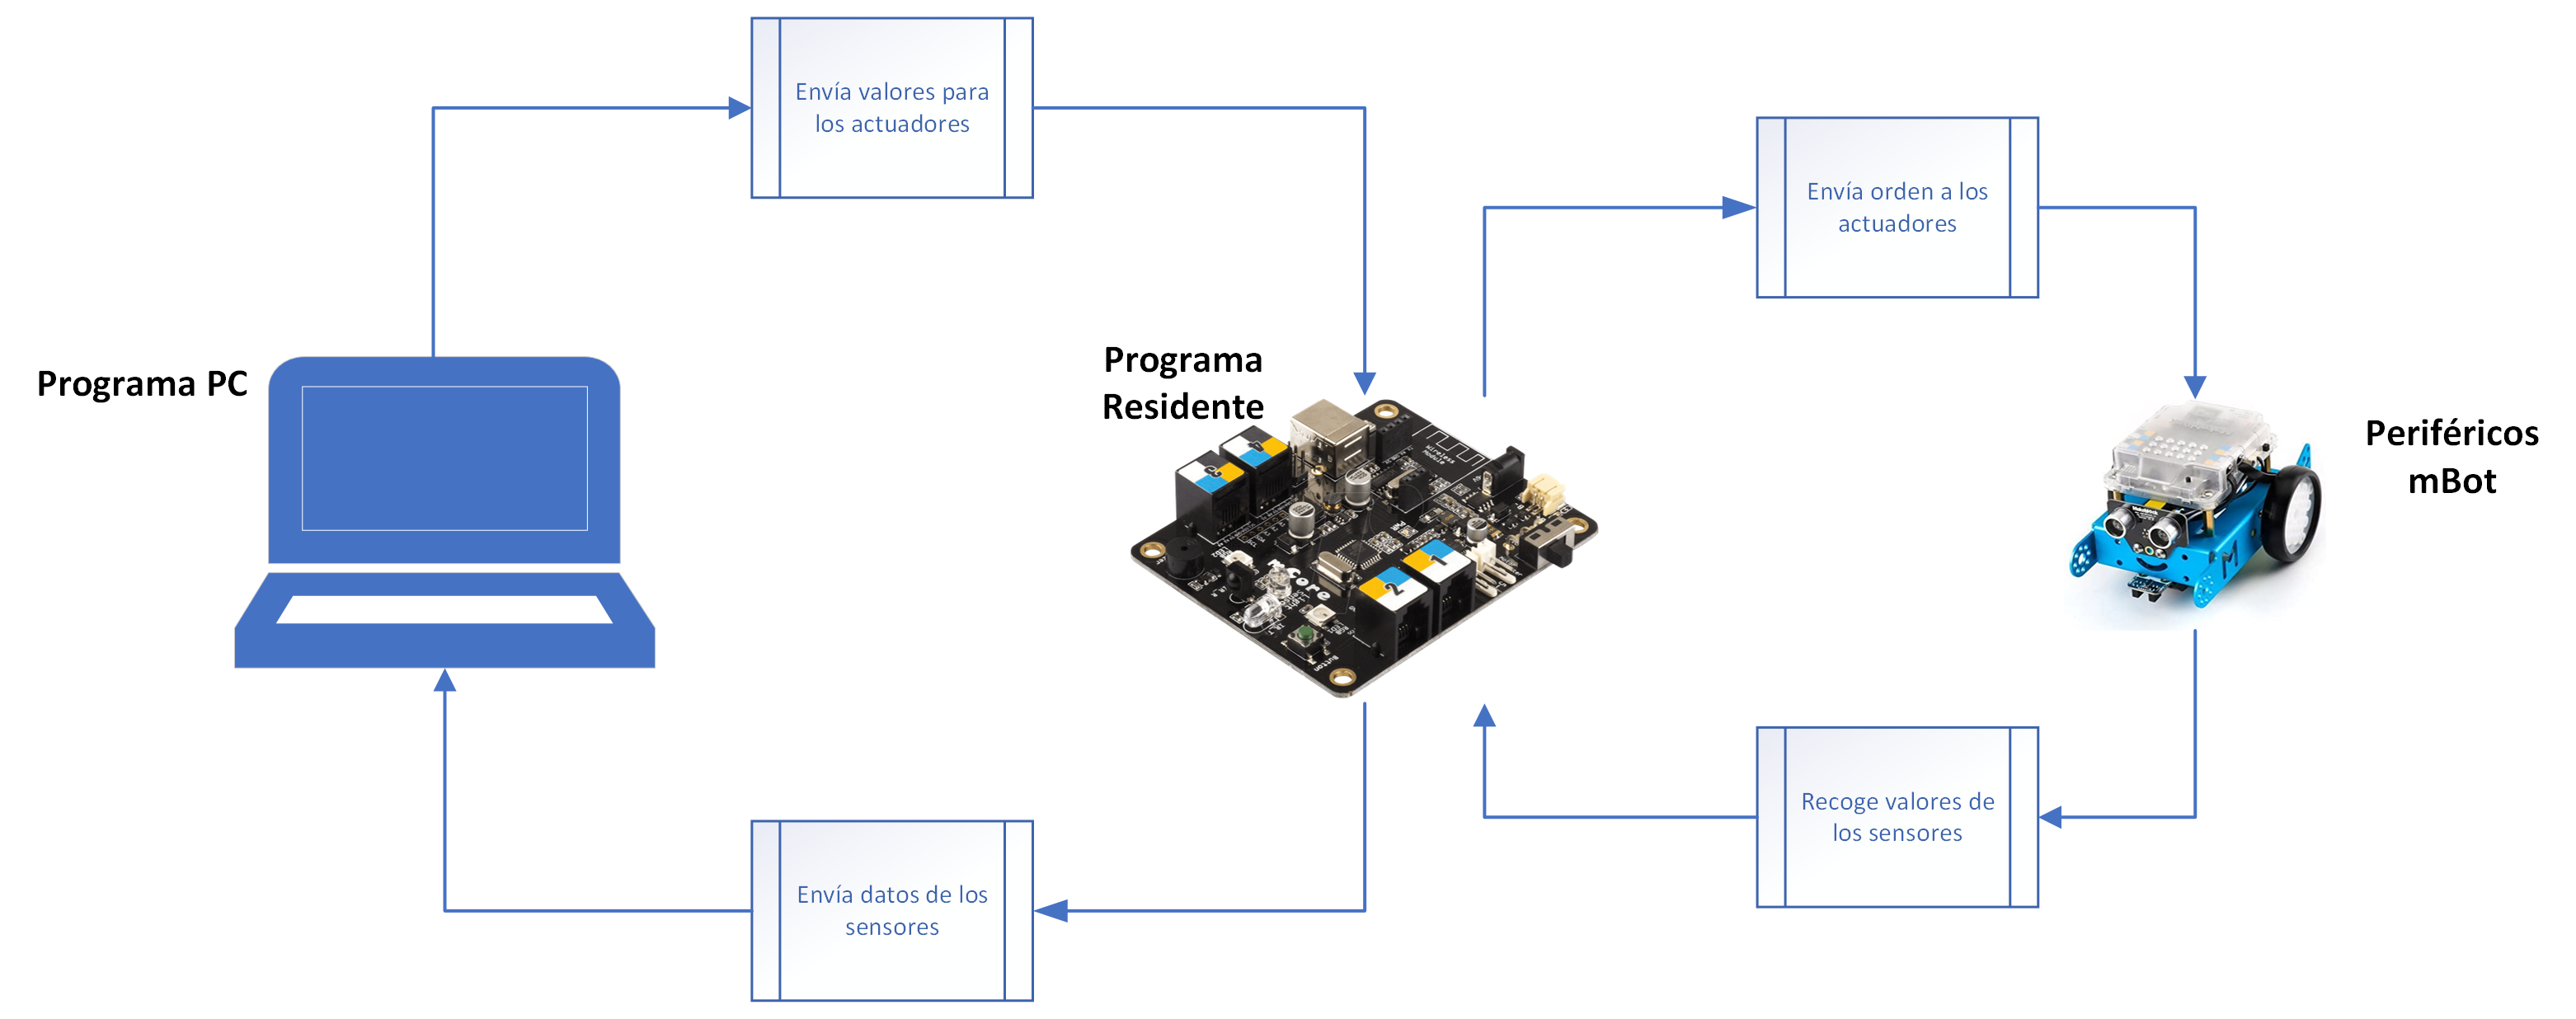
\includegraphics[scale=0.3]{flujo1.png}
	\centering
	\label{img:FlujoComunicaciones}
	\caption{Diagrama de comunicaciones entre PC y Residente}
\end{figure}

\begin{figure}[h]
	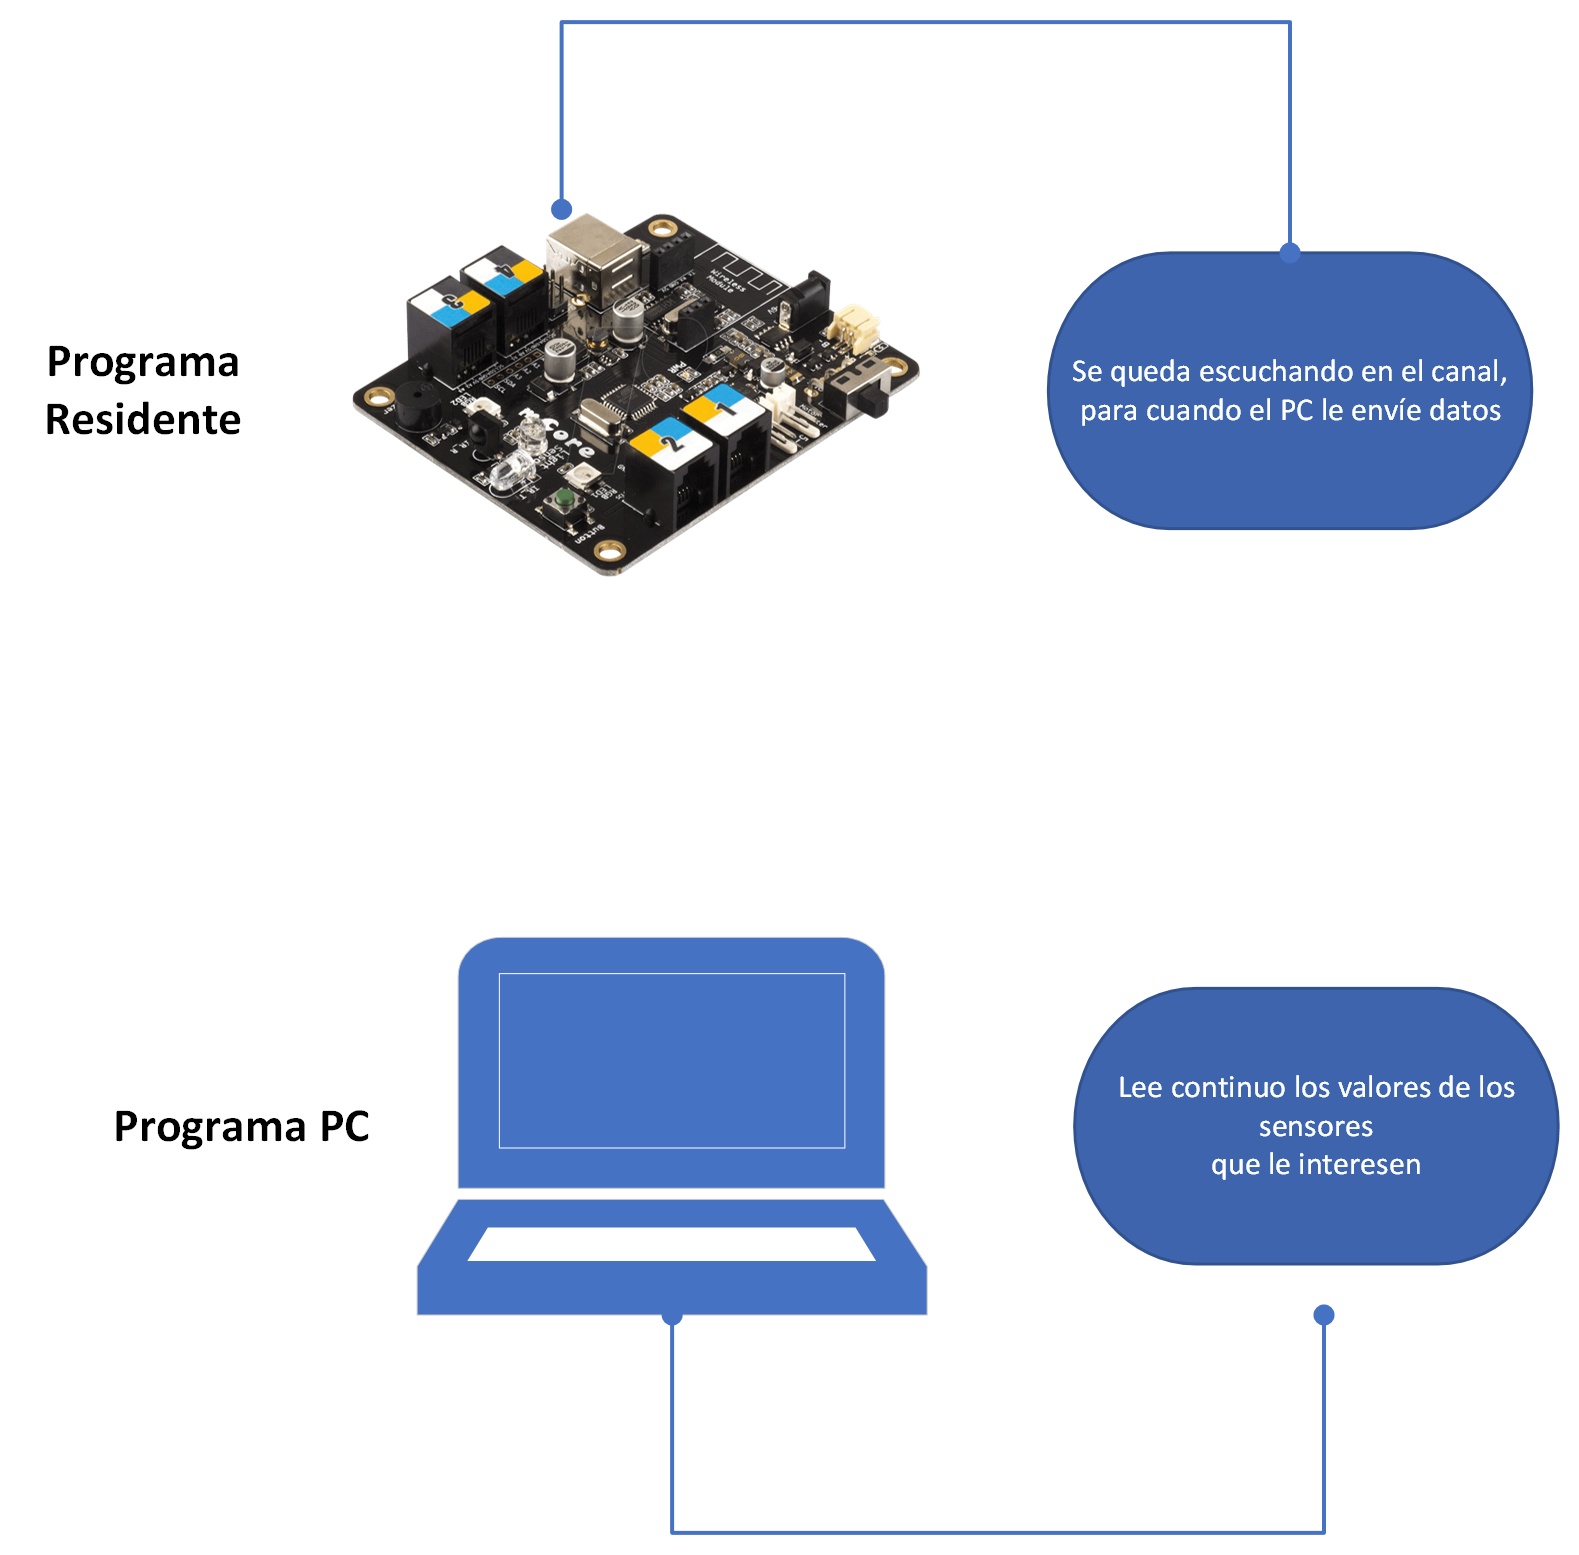
\includegraphics[scale=0.3]{flujo2.png}
	\centering
	\label{img:FlujoComunicaciones2}
	\caption{PC y Residente}
\end{figure}

Como podemos observar, ocurren varias cosas de forma paralela:
\begin{itemize}
	\item El programa residente está recogiendo los valores de los sensores, conectados a su puerto correspondiente, y los envía por el canal.
	\item El programa PC recoge los valores del sensor que le interese (dependerá del programa que queramos uno u otro).
	\item En función del valor del sensor (con respecto a un valor umbral o \textit{threshold}), el programa PC envía por el canal unos valores concretos para un actuador concreto. Lee otra vez el valor -nuevo- del sensor, por si tuviera que cambiar de decisión.
	\item El programa residente lee del canal si tiene mensajes para un actuador y, en caso afirmativo, recoge los valores y los envía al actuador correcto.
\end{itemize}

\section{Protocolo de mensajes}\label{sec:protocolomensajes}
Para que la comunicación entre el programa PC y Residente sea posible es necesario un protocolo de mensajes; es necesario asegurarse que ambas partes recojan la información correcta y sepan qué deben hacer con ella. Poniendo un ejemplo: el Programa Residente debe estar preparado para recibir datos que enviar a los actuadores. Sin embargo, cada actuador requiere datos de entrada diferentes, por tanto, debe estar preparado también para saber para qué actuador le están enviando los datos. Igualmente, el Programa PC debe estar preparado para enviar la información de forma que sea inequívoca. \\
El mismo caso se da para los sensores. El Residente tiene que enviar el dato de forma que el PC pueda saber que el dato que lee es el que necesita (no vale para lo mismo si lee el sensor de luz que el del Sigue Líneas) \\

Este sistema de codificación de los mensajes, funciona de la siguiente forma:
\begin{itemize}
	\item Sensores
	\begin{itemize}			
		\item Dado que la forma más simple, y efectiva debido a ello, de enviar datos es un string, será así como se enviará la información. Para ello, cuando se lea el dato del sensor, habrá que convertir el valor entero en un String. 
		\item A cada sensor se le asignará un número, único (un identificador), que le representará sólo a él. Así, al sensor de ultrasonidos le corresponderá un 0, al Sigue Líneas un 1, etc. 
		\item El Programa Residente, enviará la información en un único mensaje, como String, concatenando el identificador de sensor con el valor de este sensor recogido del robot, separando los dos valores con punto y coma (para diferenciarlo de una posible coma decimal).
		\item El Programa PC, cuando está leyendo, separará el mensaje por ';' y ,dependiendo del primer \textit{substring}, devolverá al programa principal el tipo de sensor en texto, para que sea amigable para un alumno. 
	\end{itemize}
	\begin{figure}[h]
		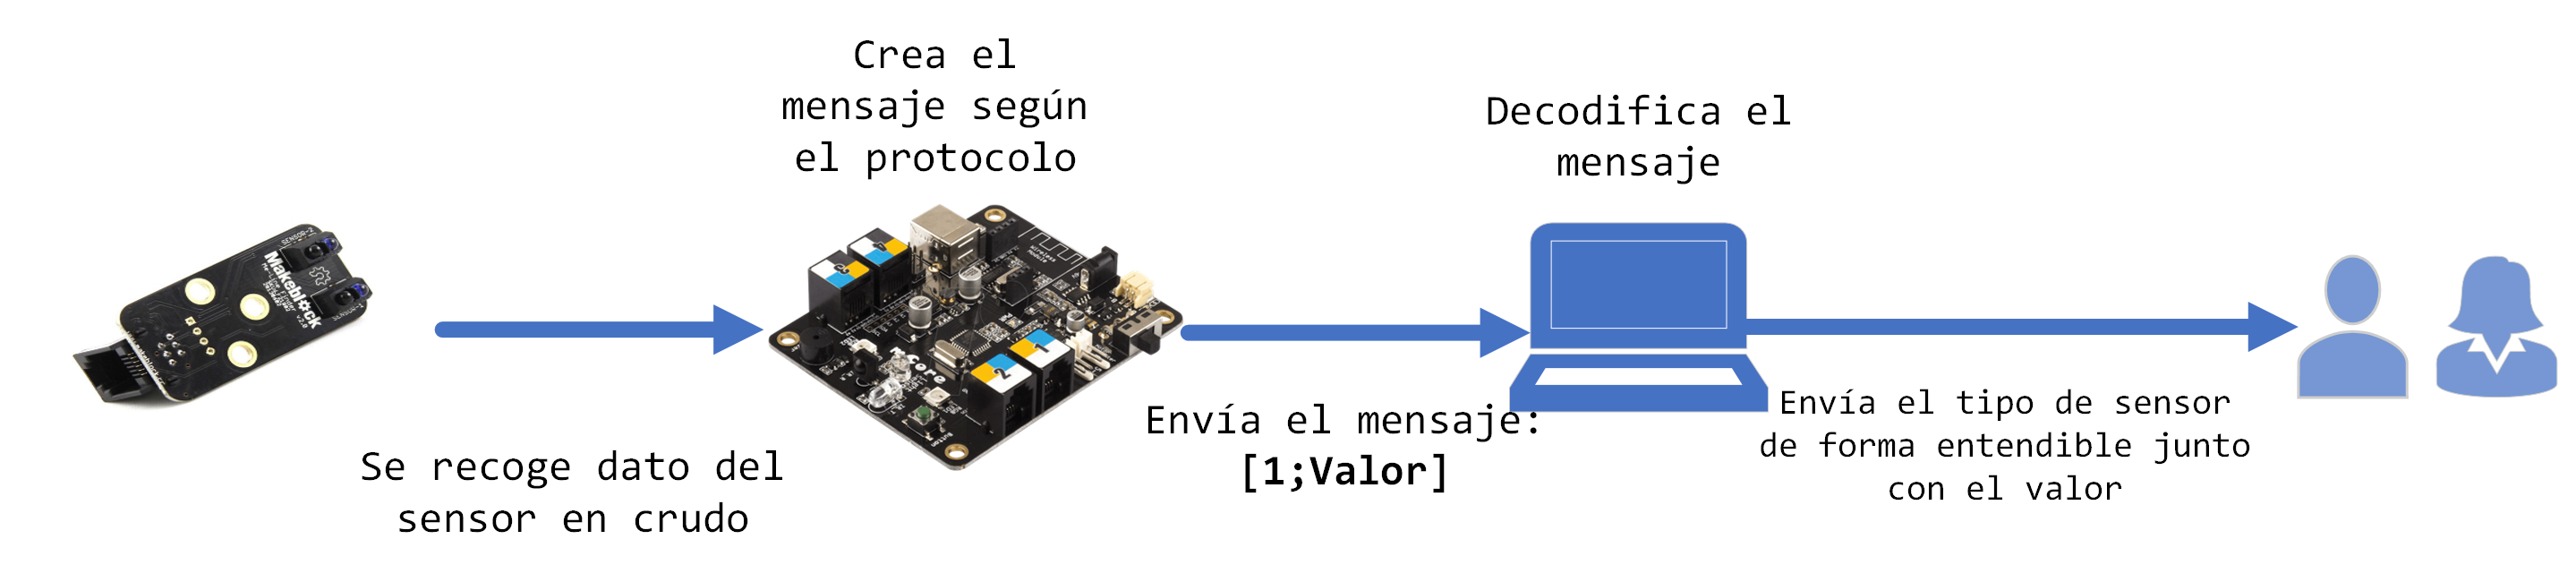
\includegraphics[scale=0.3]{mensajeSensor.png}
		\centering
		\label{img:mensajeSensor}
		\caption{Flujo de mensajes para un sensor}
	\end{figure}
	\item Actuadores
	\begin{itemize}
		\item De forma análoga, a cada actuador se le asignará un identificador numérico.
		\item El Programa PC concatenará, en un mismo mensaje, el identificador del actuador, y los datos necesarios para ese actuador (en caso de los LED, por ejemplo, el valor qué leds encender y los tres valores RGB). Igualmente, todos estos valores irán separados entre ';'. Estos valores serán decididos por el programa principal (por el programador/a).
		\item Al leer del canal, el Residente separará el primer valor por el ';' y dependiendo de qué identificador sea, leerá una cantidad de valores u otra, y enviará esos valores a un actuador u otro (convirtiéndolo primero a valor numérico).
	\end{itemize}
\begin{figure}[h]
	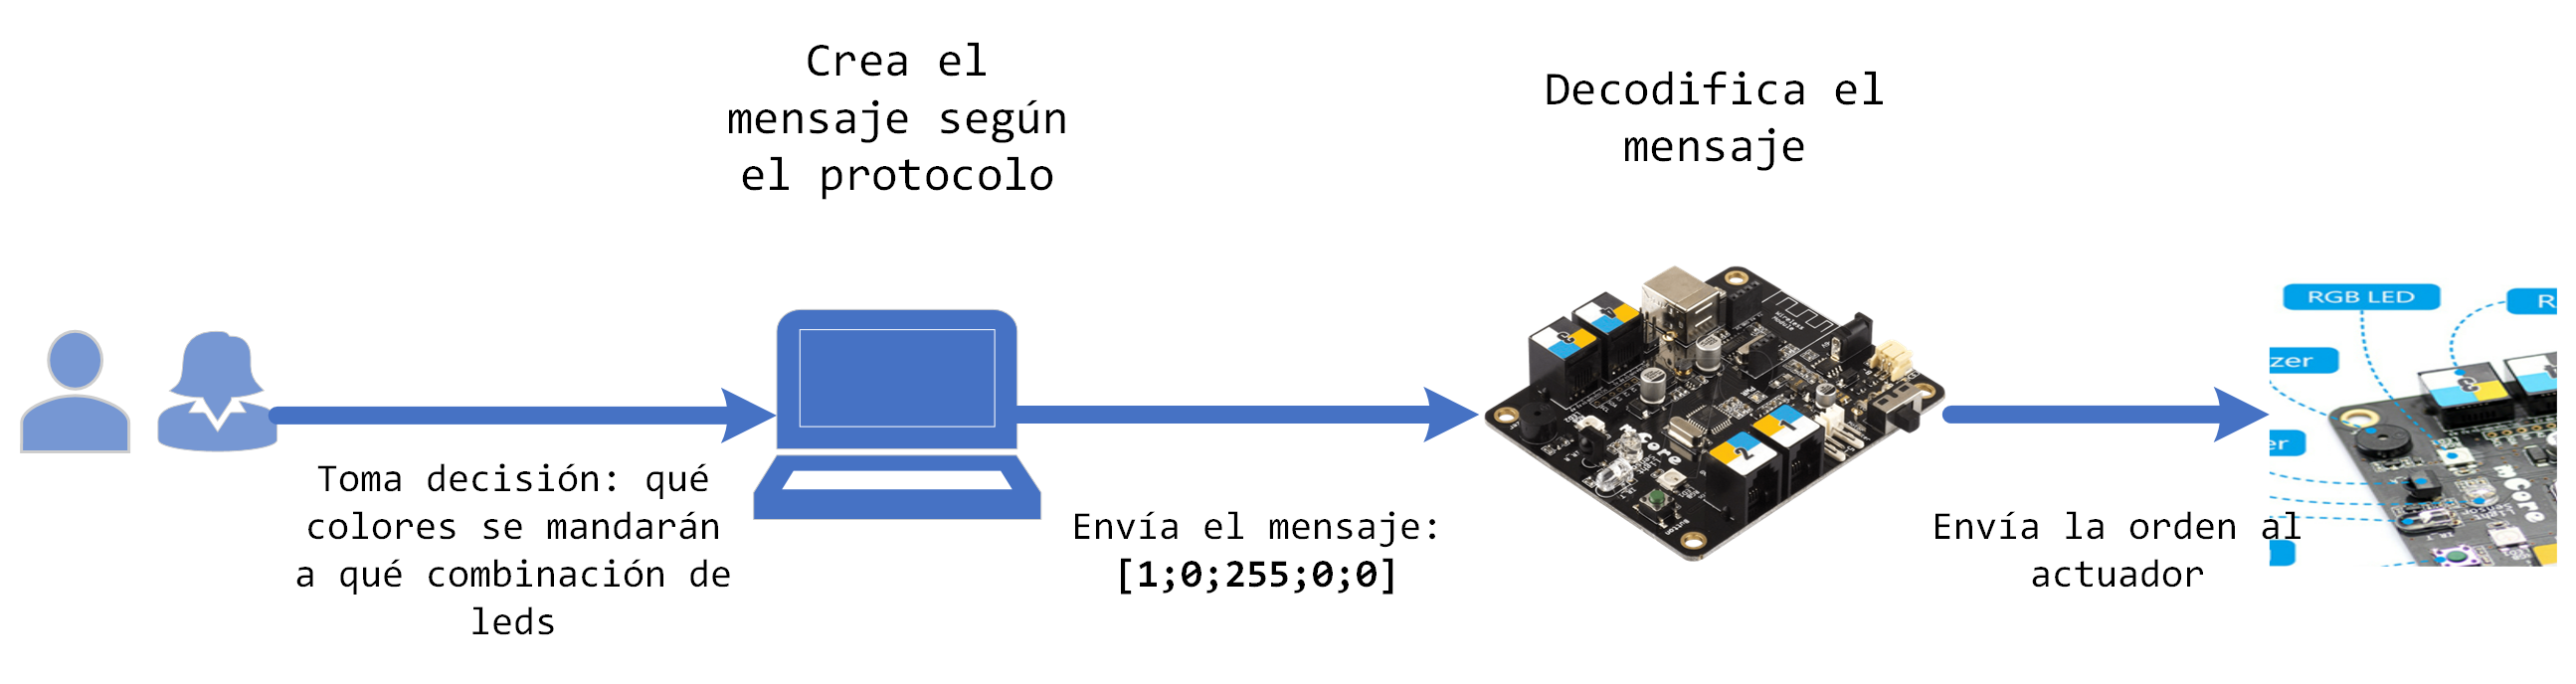
\includegraphics[scale=0.3]{mensajeActuador.png}
	\centering
	\label{img:mensajeActuador}
	\caption{Flujo de mensajes para un sensor}
\end{figure}
\end{itemize}


Con este protocolo de mensajes la funcionalidad de la plataforma PyBoKids 2.0 es fácilmente ampliable a más sensores o actuadores, puesto que los identificadores son números enteros. \\

A continuación, detallaremos la forma técnica en la que se han en la que se ha desarrollado el diseño en ambas partes, Residente y PC, explicando el acceso a los periféricos, la construcción de las bibliotecas y el manejo de este protocolo de mensajes. 
\section{Programa residente en robot}\label{sec:residente}
La biblioteca residente en Arduino se ha realizado de forma progresiva, encontrando diferentes requerimientos y necesidades a lo largo del proceso. 
\subsection{Comunicación serial}\label{subsec:SerialArduino}
En Arduino, para utilizar el protocolo Serial no es necesario cargar ningún módulo añadido, al ser un lenguaje pensado para las comunicaciones electrónicas. La inicialización de la comunicación Serial debe hacerse en la función \textit{setup} de Arduino, donde se coloca el código que debe ejecutarse sólo una vez, al comienzo de la ejecución del programa, con la velocidad en baudios deseada como parámetro.
\begin{lstlisting}[language=C,caption={Inicialización del protocolo Serial},captionpos=b]
void setup() {
  // put your setup code here, to run once:
  Serial.begin(9600);
}
\end{lstlisting}
Durante el resto del código, cada vez que se quiera escribir o leer del canal, deberá llamarse al 'Serial' que hemos iniciado. Es importante comentar que, antes de llamar a una función que lea del canal, debemos asegurarnos que hay datos que poder leer, o el programa generará un error. Por ejemplo:
\begin{lstlisting}[language=C,caption={eco en Arduino: lee del canal Serial y lo escribe},captionpos=b]
char mensaje;
void loop() {
  if (Serial.available()>0)	{
   mensaje = Serial.read();   
   Serial.println(mensaje);
  }
}
\end{lstlisting}
A la hora de leer del canal Serial (en este caso en Arduino, pero igual con cualquier herramienta) hay que tener en cuenta la cantidad de bytes que se leen cada vez. En este caso, estábamos considerando a modo de test, un sólo carácter (inicializando la variable como \textit{char})\footnote{Variable que almacena un valor de carácter, que ocupa un sólo byte de memoria, y que debe escribirse entre comillas simples:\textit{ char mensaje = 'a';}}, por lo que leemos del canal un solo byte (método \textit{read()}). Sin embargo, si quisiéramos leer un \textit{String}\footnote{Array de caracteres, escrito entre comillas dobles, y que termina en valor nulo ('0' en código ASCII): \textit{String mensaje =  "Hello String";}}, como va a ser necesario para leer los mensajes que envíe el programa PC, tendríamos que inicializar la variable como \textit{String} y leer del canal un String entero, esto es, hasta leer el valor nulo en el que éste termina.
\begin{lstlisting}[language=C,caption={eco en Arduino con un Strin},captionpos=b]
String mensaje;
void loop() {
  if (Serial.available()>0) {
   mensaje = Serial.readString();     
   Serial.println(mensaje);
  }
}
\end{lstlisting}

Dado que primero estamos considerando solamente el entorno Arduino, para poder ver el resultado de esta comunicación, usaremos el Monitor Serie del propio IDE de Arduino, que permite escribir por el canal (lo que luego leamos con \textit{serial.readString()}), y muestra lo que Arduino escribe (\textit{Serial.println()}). El código anterior produciría la siguiente ejecución:
\begin{figure}[h]
\centering	
\begin{subfigure}
	[Escribir el String que Arduino lee del canal]{
		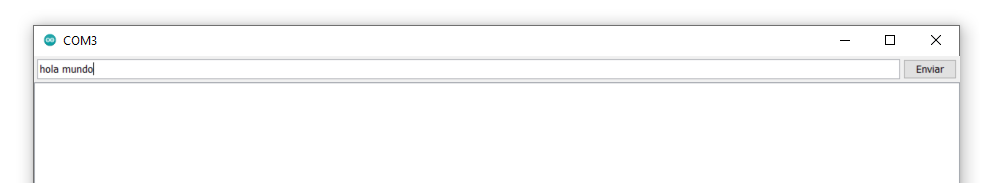
\includegraphics[width=\textwidth]{MonitorEnviar.png}
		\label{img:ComunicacionArduinoEnviar}}
\end{subfigure}
\begin{subfigure}
	[Muestra el String que Arduino ha escrito en el canal]{
		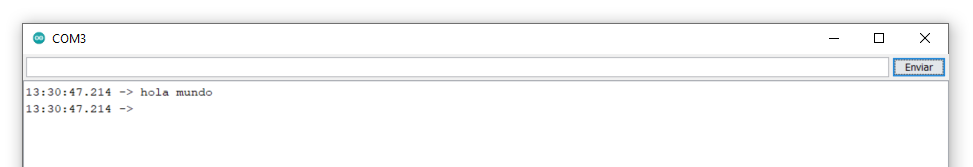
\includegraphics[width=\textwidth]{MonitorRespuesta.png}
		\label{img:ComunicacionArduinoLeer}}
\end{subfigure}
\label{img:ComunicacionArduinoMonitorSerie}
\caption{Visualización del eco de Arduino en el Monitor Serie de Arduino IDE}
\end{figure}

\subsection{Uso de sensores y actuadores}\label{subsec:sensoresyactuadoresArduino}
Una vez comprobadas las comunicaciones, continuamos con los actuadores y sensores del robot. Como se ha explicado en el apartado \ref{subsec:arduino} de Arduino, es necesario cargar los módulos correspondientes a la placa mCore. Una vez incluido el paquete, podremos utilizar los métodos de inicialización, lectura de sensores, envío de órdenes a los actuadores, etc. Este módulo contiene toda la información que necesitan los diferentes componentes (tipos de valores de entrada o de retorno, diferentes métodos, etc), incluidos ejemplos en los que poder apoyarnos. A continuación describiremos como se utilizan los diferentes actuadores y sensores en Arduino, siendo este paso necesario para crear la biblioteca ''Residente''.\\
\begin{itemize}
\item Actuadores: Como cualquier variable, los actuadores requieren de una inicialización; esta inicialización de variables corresponden al principio del programa, para poder utilizar la variable en las funciones principales. Luego, depende de qué actuador sea, requerirá de un tipo u otro de valor de entrada:
\begin{description}
	\item [Motores] Los motores de la placa mCore deben inicializarse cada uno por separado; al darles nombres diferentes podremos enviar la orden al motor correcto (por ejemplo, para girar el robot, no debe enviarse la misma orden al motor derecho que al izquierdo, sino invertir el sentido de uno de ellos, dependiendo de en qué dirección se quiera girar). 
	\begin{lstlisting}[language=C,caption={Inicializar motores Mbot},captionpos=b]	
		MeDCMotor motorIzdo(M1);
		MeDCMotor motorDcho(M2);	
	\end{lstlisting}
	El valor de entrada para la velocidad es un valor entero (tipo \textit{int}), entre [-255,255], siendo los valores negativos para una velocidad de retroceso. En este caso, para que los motores se paren, no se les enviaría un valor de 0 sino que tiene un método propio.	
	\begin{lstlisting}[language=C,caption={Uso de motores Mbot},captionpos=b]		
	motorIzdo.run(100);
	motorDcho.run(100);
	delay (100);
	motorIzdo.stop();
	motorDcho.stop();	
	\end{lstlisting}

	\item [Leds integrados]  En este caso, la inicialización del led requiere el puerto (integrado de la placa) y un slot (de número de leds). Por tanto:
	\begin{lstlisting}[language=C,caption={Inicializar leds},captionpos=b]	
	const int PORT = 7;
	const int SLOT = 2;
	MeRGBLed led(PORT, SLOT);	
	\end{lstlisting}
	Los valores necesarios para los leds se han descrito en la sección de Actuadores \ref{subsec:actuadores}; Arduino requiere primero enviar la configuración de colores, y después mostrar esa configuración. En este caso, para apagarlos, sí se envía un valor de 0 para los tres valores RGB.
	\begin{lstlisting}[language=C,caption={Uso de los leds},captionpos=b]	
	led.setColor(ledsInt,redInt,greenInt,blueInt);
	led.show();	
	\end{lstlisting}

	\item [Zumbador] Como sólo hay un zumbador en la placa, y está integrado en ella, no es necesario ningún puerto. Para que emita la nota deseada, es necesario un valor entero para la frecuencia y otro para la duración (en milisegundos):
	\begin{lstlisting}[language=C,caption={Uso del zumbador},captionpos=b]	
	MeBuzzer buzzer;
	void loop() {
	 buzzer.tone(87,3000);
	 delay(100);
	 // stop the tone playing:
	 buzzer.noTone();
	}
	\end{lstlisting}
\end{description}
\item Sensores: Todos los sensores en Arduino tienen un método de lectura, además del de inicialización. Si queremos almacenar el valor recogido en una variable, Arduino requiere que ésta sea declarada también.
\begin{description}
	\item [Sensor de ultrasonidos] Al no ser un sensor integrado a la placa, es necesario que se especifique en qué puerto se ha conectado. Éste devuelve la distancia, en centímetros (como valor entero), a la que se encuentra un obstáculo.
	\begin{lstlisting}[language=C,caption={Sensor de distancia},captionpos=b]	
	MeUltrasonicSensor ultraSensor(PORT_3);
	void loop() {
	 int DistanceValue = ultraSensor.distanceCm();
	 Serial.println(DistanceValue);
	}
	\end{lstlisting}
	\item [Sensor de luz] El puerto especificado en la llamada al método, aunque integrado en la placa, especifica el pin interno al que está conectado. Devuelve un valor entero, de cantidad de luz. En este caso, para poder utilizar un valor de \textit{threshold} necesitaremos saber qué valor de luminosidad aproximada tiene la habitación (no tiene por qué ser siempre la misma)
	\begin{lstlisting}[language=C,caption={Sensor de luz},captionpos=b]	
	MeLightSensor lightSensor(PORT_6);
	void loop() {
	 int LigthValue = lightSensor.read();
	 Serial.println(LigthValue);
	}
	\end{lstlisting}
	\item [Sensor infrarrojo] Requiere también especificar a qué puerto se le ha conectado, devolviendo de la llamada de lectura un valor entero correspondiente a qué combinación de sensores sigue líneas están tapados o no (explicados en la sección de Actuadores (\ref{subsec:actuadores}))
	\begin{lstlisting}[language=C,caption={Sensor siguelíneas},captionpos=b]	
	MeLineFollower SigueLineas(PORT_1); 
	void loop() {
	 int LineFollowerValue = SigueLineas.readSensors();
	 Serial.println(LineFollowerValue);
	}
	\end{lstlisting}
\end{description}
\end{itemize}

\subsection{Protocolo de mensajes}\label{subsec:mensajesArduino}

Por último, explicaremos cómo se ha desarrollado en el lado Arduino el protocolo de mensajes cuyo diseño está detallado en  \ref{subsubsec:protocolomensajes}. \\
Como se ha comentado, cada sensor y cada actuador tienen un identificador asignado.
\begin{table}[h]
	\centering
	\begin{tabular}{ c | c }
		Periférico & Identificador \\
		\hline			
		Sensor de Distancia &  0\\
		Sensor Sigue Líneas & 1 \\
		Sensor de Luz & 2\\
		\hline
		Leds integrados & 0\\
		Motores & 1\\
		Zumbador & 2 \\

	\end{tabular}
\caption{Relación de periféricos del mBot con su identificador}
\label{table:identificadoresperifericos}
\end{table}
No supone ningún peligro de discrepancia que entre sensores y actuadores tengan identificadores repetidos, ya que los mensajes que lo contienen no van en la misma dirección: los mensajes de los sensores son enviados por el programa Residente y leídos por el programa PC, y los mensajes de los actuadores, del revés.\\

Para utilizar estos mensajes de forma real, necesitaremos en nuestra biblioteca funciones para leer los correspondientes a los sensores, y  componer los de actuadores. \\
Para componer un mensaje para un sensor, las consideraciones a tener en cuenta son: 
\begin{itemize}
	\item Debemos enviar un String, por lo que deberemos convertir a String los valores numéricos.
	\item Los identificadores no pueden cambiarse, por lo que los dejaremos embebidos en el código.
	\item El separador será por punto y coma, para evitar errores en la lectura. Si fuera una coma, podría confundirse con un posible valor numérico decimal del sensor.
\end{itemize} 
\begin{lstlisting}[language=C,caption={Envío de mensajes para los sensores},captionpos=b]
void Send_DistanceMessage () {
	int DistanceValue = ultraSensor.distanceCm();
	String DistanceValueString = String(DistanceValue);
	String DistanceMessage = "0;" + DistanceValueString; 
	Serial.println(DistanceMessage);
}

void Send_LineFollowerMessage () {
	int LineFollowerValue = SigueLineas.readSensors();
	String LineFollowerString = String(LineFollowerValue);
	String LineFollowerMessage = "1;" + LineFollowerString; 
	Serial.println(LineFollowerMessage);
}

void Send_LigthSensorMessage () {
	int LigthValue = lightSensor.read();
	String LigthString = String(LigthValue);
	String LigthMessage = "2;" + LigthString; 
	Serial.println(LigthMessage);
}
\end{lstlisting}

En el caso de los actuadores, dado que son el mensaje ''que llega'' ya formado, para leer debemos:
\begin{itemize}
	\item El mensaje que llega es un String.
	\item Debemos separar ese String por el separador, punto y coma, y almacenar los valores en variables temporales. 
	\item El primer valor que se extraiga, corresponde al tipo de actuador, y dependerá de éste qué lectura del resto del mensaje tenga que hacerse. 
	\item Los valores que deben enviarse como parámetros a los actuadores deberán convertirse en valor numérico, pues es así como lo espera el actuador. 
\end{itemize} 
\begin{lstlisting}[language=C,caption={Decisión sobre los actuadores con el primer valor del mensaje},captionpos=b]
int indexActuator = mensaje.indexOf(';');
String Actuator = mensaje.substring(0,indexActuator);
String mensajeActuador = mensaje.substring(indexActuator+1);
if (Actuator == "0") {
	read_LedsMessage(mensajeActuador);
} else if (Actuator == "1") {
	read_MotorsMessage(mensajeActuador);
} else if (Actuator == "2") {
	read_BuzzerMessage(mensajeActuador);
}
\end{lstlisting}
\begin{lstlisting}[language=C,caption={Lectura de mensajes de los actuadores},captionpos=b]
void read_LedsMessage (String mensaje) {
	int IndexLeds = mensaje.indexOf(';');
	String leds = mensaje.substring(0, IndexLeds);
	int IndexRed = mensaje.indexOf(';', IndexLeds+1); 
	String red = mensaje.substring(IndexLeds+1, IndexRed+1);
	int IndexGreen = mensaje.indexOf(';', IndexRed+1);
	String green = mensaje.substring(IndexRed+1, IndexGreen+1);
	String blue = mensaje.substring(IndexGreen+1,-1); 
	int ledsInt = leds.toInt();
	int redInt = red.toInt();
	int greenInt = green.toInt();
	int blueInt = blue.toInt();
	led.setColor(ledsInt, redInt, greenInt, blueInt);
	led.show();
}	
void read_MotorsMessage (String mensaje) {
	int IndexIzdo = mensaje.indexOf(';');
	String izdo = mensaje.substring(0, IndexIzdo);
	String dcho = mensaje.substring(IndexIzdo+1,-1);	
	int izdoInt = izdo.toInt();
	int dchoInt = dcho.toInt();
	motorIzdo.run(izdoInt);
	motorDcho.run(dchoInt);
}
void read_BuzzerMessage (String mensaje) {
	int IndexNote = mensaje.indexOf(';');
	String note = mensaje.substring(0, IndexNote);  
	String duration = mensaje.substring(IndexNote+1,-1);
	int NoteInt = note.toInt() ;
	int DurationInt = duration.toInt();	
	int durationValue = 1000 * DurationInt;  
	int pauseBetweenNotes = durationValue * 1.30;
	buzzer.tone(NoteInt,durationValue);
	delay(pauseBetweenNotes);
	buzzer.noTone();
}	
\end{lstlisting}

\par Como apunte añadido, y dado que la placa Arduino no se ''apaga'' dejando a neutro todos los valores electrónicos (si apagamos el robot teniendo los led encendidos, cuando se vuelva a encender, lo hará con ellos encendidos), hacía falta una forma de poder apagar todo. En esta biblioteca Residente tendremos las funciones correspondientes para dejar apagados cada actuador con sus valores correspondientes:

\begin{lstlisting}[language=C,caption={Apagado de los actuadores},captionpos=b]
void Stop_Motors () {
	motorIzdo.stop();
	motorDcho.stop();
}

void Stop_Leds () {
	led.setColor(0, 0, 0, 0);
	led.show();
}

void Stop_Buzzer () {
	buzzer.noTone();
}	
\end{lstlisting}

Esta funcionalidad de ''apagado'' se pedirá con un mensaje desde el programa PC, que controlaremos en Arduino al principio de lectura del mensaje:

\begin{lstlisting}[language=C,caption={Apagado de los actuadores},captionpos=b]
String mensaje = Serial.readString();
if (mensaje.equalsIgnoreCase("quit")) {
	Stop_Motors();
	Stop_Leds();
	Stop_Buzzer();
	exit(0);
}
\end{lstlisting}

Una vez conocido el funcionamiento de los componentes del mBot, hemos podido abstraer este conocimiento y desarrollar las funciones que compondrán esta biblioteca Arduino. Estas funciones crearán la estructura del programa residente de forma que funcione independientemente de qué datos se le envíen desde el programa PC.

\section{Programa PC}\label{sec:pc}
La finalidad del Programa PC es tener una biblioteca de funciones que contengan la lógica de conexión, lectura, escritura, etc, y que la escondan a los alumnos, teniendo ellos que preocuparse solamente de llamar a una función con un nombre amigable. A continuación describiremos los puntos importantes que se han necesitado en la preparación de esta biblioteca.
\subsection{Comunicación Serial}\label{subssec:serialPython}

En este caso, es necesario incluir el módulo Serial al principio del programa de Python. Para iniciar una comunicación Serial, al igual que con Arduino, es necesaria la velocidad en baudios a la que conectarse (como dijimos, debe ser la misma a la que se ha abierto la comunicación en la parte de Arduino); además es necesario el puerto al que está conectado el robot (de forma parecida a la que se especificaba en el Arduino IDE) y un tiempo de \textit{timeout} para el que, si no se ha establecido la comunicación, se eleva una excepción (que se deberá recoger con un bloque de \textit{try..catch}). 
\begin{lstlisting}[language=python,caption={Función de la biblioteca Python para abrir el puerto serie},captionpos=b]	
def open_PortSerial (port):
	try:
		serialAux = serial.Serial(115200, port, timeout=1)
		serialAux.setDTR(False)
		sleep(1)
		serialAux.flushInput()
		serialAux.setDTR(True)
		sleep (1)
		return serialAux
	except serial.SerialException:
		sys.stderr.write("Error al abrir puerto (%s)\n")
		sys.exit(1)
\end{lstlisting}

La velocidad a la que funcione la comunicación Serial se ha establecido finalmente en 115200 baudios ya que, de forma experimental, al añadir los sensores fue necesario subir el valor para mantener la comunicación de forma útil. Este valor se establece como constante, para asegurarnos que es el mismo valor en las dos partes PC y Residente. 

\paragraph {Leer del canal} 
Para leer del canal, deberemos tener en cuenta igualmente la cantidad de información que queramos leer. En general, como estaremos leyendo mensajes tipo String, Python contiene (como Arduino) la función de lectura de una línea completa (hasta fin de línea). 
\begin{lstlisting}[language=python]
serial.readline() #leer hasta EOL		
\end{lstlisting}
Sin embargo, es posible leer un solo byte (como en el caso de leer un solo carácter), o una cantidad de bytes especificada.

Dado que el String leído con el valor de un sensor, lo ha enviado Arduino y ha atravesado el canal, es necesario decodificarlo para obtener un String sin los caracteres de retorno de carro, end of line, etc. Si no, no podríamos utilizar como número ese valor, ya que al intentar convertirlo desde String, no debe tener ningún otro carácter.
\begin{lstlisting}[language=python]	
Data = serial.readline()
decoded = Data.decode()
sensorValue = float(decoded)
\end{lstlisting}
	
	
\paragraph {Escribir en el canal} Al igual que para leer, para escribir en el canal y asegurarnos que en al programa residente le llegan datos que sea capaz de interpretar, el envío de datos (texto) debe hacerse forzando la codificación en UTF-8.
\begin{lstlisting}[language=python]
Data = "Hello World"
serial.write(bytes(Data, 'utf-8'))
\end{lstlisting}

Estas decisiones de codificaciones, tanto para escribir como para leer del canal, son el resultado de pruebas entre uno y otro lado (Arduino - Python), con varios tipos de datos y de formas de leer del canal (bytes, Strings, etc), con la finalidad de asegurar que ambos lados pueden establecer una comunicación con éxito y que las opciones necesarias están recogidas.

\subsection{Protocolo de mensajes}\label{subsec:mensajesPython}
En el caso de la biblioteca Python, no debemos preocuparnos de los sensores y actuadores como Hardware, ya que el programa PC no lee directamente de ellos, sino que se comunica con la placa base (con el programa Residente). Por tanto, deberemos establecer la lectura y envío de los mensajes, en este caso del revés que en el lado Residente: la lectura y decodificación serán para los sensores, y el envío para los actuadores. La biblioteca contendrá toda esta funcionalidad ''escondida'' para que los alumnos utilicen simplemente funciones con nombres autoexplicativos, tales como 'turnOnLeds' o 'readSensor'.\\
Tendremos en cuenta los siguientes puntos:
\begin{itemize}
	\item Los identificadores para mensajes y actuadores son, obviamente, los mismos que en el programa Residente, mostrados en la tabla \ref{table:identificadoresperifericos}.
	\item Enviaremos y recibiremos los mensajes como String.
	\item Para enviar un mensaje a un actuador, el identificador será unívoco, e irá embebido en el código.
	\item Igualmente, los separadores de los mensajes serán por punto y coma, pues es como lo espera el lado Residente.
	\item A la hora de recibir un mensaje, se utilizará el separador ';' para, en primera instancia, decidir qué sensor le corresponde y enviarlo al programa principal (el que programan los estudiantes) en texto, junto con el valor numérico.
\end{itemize}
La forma en la que codificamos los mensajes para los actuadores es la siguiente:
\begin{lstlisting}[language=python,caption={Funciones en la biblioteca PC para la codificación de mensajes de los actuadores},captionpos=b]
def create_Message_Led (list):
	mensaje = f"0;{list[0]};{list[1]};{list[2]};{list[3]}"
	return mensaje
	
def create_Message_Motor(list):
	mensaje = f"1;{list[0]};{list[1]}"
	return mensaje
	
def create_Message_Buzzer(list):
	mensaje = f"2;{list[0]};{list[1]}"
	return mensaje
\end{lstlisting}

Estas funciones, nos devuelven el mensaje creado listo para enviar.Sin embargo, estas funciones de codificación son un nivel de abstracción, no de uso para los estudiantes. Para enviar el mensaje, utilizamos las funciones que verán y utilizarán los alumnos y alumnas desde el programa principal:
\begin{lstlisting}[language=python,caption={Funciones en la biblioteca PC para el envío de mensajes a los actuadores},captionpos=b]
def turnOn_Leds(list,serial):
	mensaje = create_Message_Led(list)
	send_Message(mensaje,serial)

def turnOn_Buzzer(list,serial):
	mensaje = create_Message_Buzzer(list)
	send_Message(mensaje,serial)

def turnOn_Motors(list,serial):
	mensaje = create_Message_Motor(list)
	send_Message(mensaje,serial)
\end{lstlisting}

Estas funciones, ya sí, son las que se utilizarán como nivel de abstracción ''cero'', con un lenguaje y uso adaptado a los estudiantes:
\begin{lstlisting}[language=python,caption={Uso de los actuadores desde el Programa Principal},captionpos=b]
turnOn_Leds([0,255,0,0],serial)
turnOn_Motors([100,100],serial)
turnOn_Buzzer([131,3],serial)
\end{lstlisting}

A la hora de leer los mensajes de los actuadores, y al igual que con los actuadores, tendremos una función para leer del canal, que separará por tipo de sensor y devolverá los valores al programa principal ocultando las abstracción de los identificadores, conversión de tipos o del control de errores, necesarias en cualquier caso:
\begin{lstlisting}[language=python,caption={Lectura de los sensores en la biblioteca PC},captionpos=b]
def read_Sensor (serial):
	Data = serial.readline()
	try:
		decoded = Data.decode()
	except (UnicodeDecodeError):
		return -1 
	
	List = decoded.split(';')
	try:
		sensorValue = float(List[1])
	except (ValueError,IndexError):
		return -1 
	if (int(List[0]) == 0):
		return ["distance",sensorValue]
	elif (int(List[0]) == 1):
		return ["siguelineas",sensorValue]
	elif (int(List[0]) == 2):
		return ["luz",sensorValue]
\end{lstlisting}
Como se puede ver, en caso de añadir sensores a la plataforma, estas funciones están preparadas para ser ampliables fácilmente.\\
En el programa principal, usaremos la función con un control de decisión sobre el sensor que necesitemos:
\begin{lstlisting}[language=python,caption={Lectura de sensores en el Programa Principal},captionpos=b]
sensorMessage = read_Sensor(serial)
if (sensorMessage == -1):
	pass
else:
	if (sensorMessage[0] == 'distance'):
		print ("distance")
	elif (sensorMessage[0] == 'siguelineas'):
		print ("siguelineas")
	elif (sensorMessage[0] == 'luz'):
		print ("sensor de luz")
		
\end{lstlisting}

\par En caso de querer apagar completamente el robot y dejar a los actuadores con los valores en neutro para terminar el programa (que no en caso de querer parar un actuador en concreto dentro del programa principal), en el lado Arduino hemos explicado que tenemos una función para 'apagar' cada actuador. Por lo tanto, en este Programa Python tendremos la función 'Quit', que pedirá al residente apagarlo todo y parar, y que será el mensaje que decodifique el programa residente. Como hemos comentado en la sección anterior respecto a la forma de codificar texto en el canal, esta función \textit{quit}, siento el nivel de abstracción ''cero'' que se utiliza en el Programa Princial, tendrá oculta la funcionalidad de escribir:

\begin{lstlisting}[language=python,caption={Mensaje \textit{terminate} para los actuadores},captionpos=b]
def send_Message (message, serial):
	serial.write(bytes(message, 'utf-8'))
def send_Quit(serial):
	send_Message("quit",serial)
\end{lstlisting}

El uso de esta función dependerá de qué forma estemos programando el programa principal. Si, por ejemplo, estuviéramos leyendo de teclado y controlando el flujo con esas lecturas, podríamos mandar la orden directamente si así lo ''ordena'' la petición por teclado. También la usaremos, como hemos dicho, para terminar un programa de forma normalizada. Sin embargo, si tenemos el flujo ocupado leyendo de los sensores, no podemos estar leyendo del teclado a la vez. Podríamos utilizar un segundo hilo de ejecución (\textit{thread}), pero encontramos que ralentizaba la ejecución (importante en la lectura de los sensores) además de ser un concepto bastante más complejo para enseñárselo a un alumno o alumna que acabe de empezar a programar. La forma más efectiva por su simplicidad es capturar el terminar la ejecución en Python (Ctrl + C en Windows) y enviar ese mensaje \textit{quit} antes de terminar la ejecución de forma controlada, en vez de con el error \textit{Crtl + C}. \\

\begin{lstlisting}[language=python,caption={Ejemplo de finalización de programa con control de flujo},captionpos=b]
print ("Type 'quit' for stopping or enter to continue")
cadena=input()
if (cadena.lower() == 'quit'):
	send_Message(cadena,serial)
	
\end{lstlisting}

\newpage
\begin{lstlisting}[language=python,caption={Ejemplo de finalización de programa con control de errores},captionpos=b]
while 1:
	try:
		sensorMessage = read_Sensor(serial)    
		if (sensorMessage == -1):
			continue
		else:
			if (sensorMessage[0] == 'distance'):
				print ("distance")
	except KeyboardInterrupt:
		send_Quit(serial)
		break
\end{lstlisting}


La idea de controlar los errores es más sencilla de enseñar a los alumnos, aunque al principio del curso se les ayudará poniendo el bloque directamente en un programa ''esqueleto'', base para sus programas. Esto se explicará en profundidad en el Capítulo \ref{cap:aplicationEducativa}.

\section{Validación experimental}\label{sec:resultado}
En esta sección explicaremos con un ejemplo práctico cómo se juntan los dos programa, Residente y PC, y cómo se utilizan las dos bibliotecas. \\

\begin{figure}[h]
	\centering
	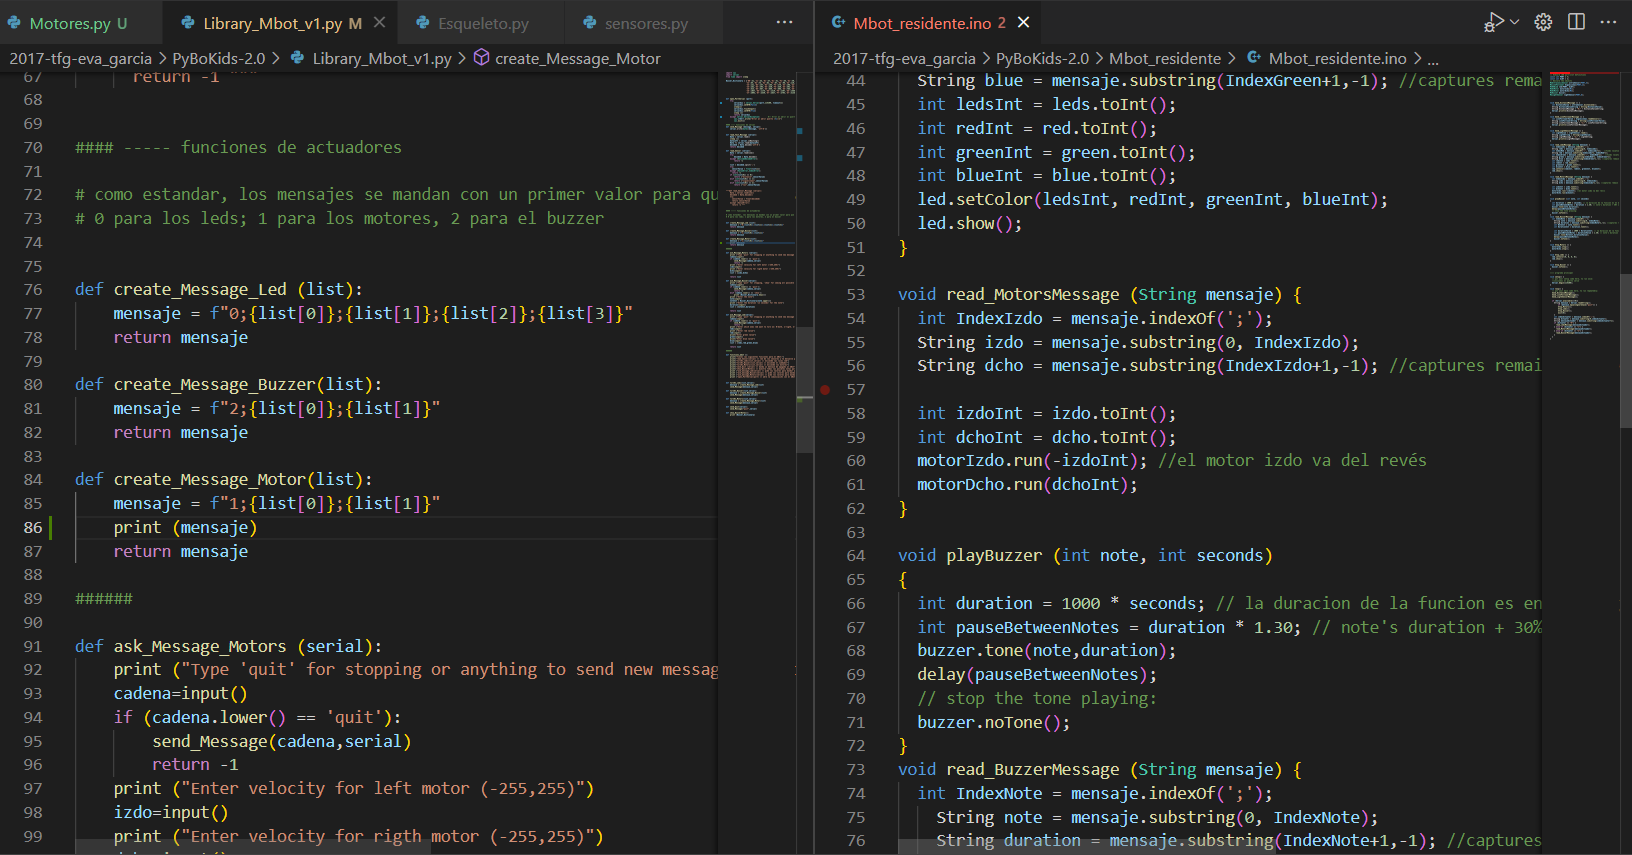
\includegraphics[scale=0.4]{programas.png}
	\label{img:Mix}
	\caption{Programa PC y Residente}
\end{figure} 
\vspace{1cm}
Utilizaremos como ejemplo de uso de las bibliotecas un ejercicio simple, utilizado durante el proceso de desarrollo de las bibliotecas, en el que se piden por pantalla las velocidades para los motores, y se manda el mensaje al programa Residente.\\
En este ejemplo, el programa principal tiene el siguiente código:
\begin{lstlisting}[language=python,caption={Ejemplo de uso de PyBoKids 2.0},captionpos=b]
import serial
from time import sleep
from Library_Mbot_v1 import *

print ("Usar los motores (M1 y M2) componiendo el mensaje completo para mandar exactamente los valores")
serial = open_PortSerial('com3')

while True:
	try:
		print ("Send new message or quit?")
		cadena=input()
		if (cadena.lower() == 'quit'):
			send_Quit(serial)
			break
		print ("Enter velocity for left motor (-255,255)")
		izdo=input()
		print ("Enter velocity for rigth motor (-255,255)")
		dcho=input()
		turnOn_Motors([izdo,dcho],serial)
	except KeyboardInterrupt:
		send_Quit(serial)
		break

serial.close()
\end{lstlisting}

Para visualizar el correcto funcionamiento del mensaje, imprimimos el mensaje, codificado, por pantalla. Aunque este código de depuración no estuviera en la versión final de la biblioteca de Python, sí ha sido útil y necesario durante el proceso de su desarrollo:

\begin{lstlisting}[language=python,caption={Uso de la bibliotca durante su desarrollo, con depuración de código},captionpos=b]
	def create_Message_Motor(list):
		mensaje = f"1;{list[0]};{list[1]}"
		print (mensaje)
		return mensaje
\end{lstlisting}

\begin{figure}[h]
	\centering
	\includegraphics[scale=0.6]{ejemploEjercicio.png}
	\label{img:ProgramaPrincipal}
	\caption{Programa Principal}
\end{figure} 
 
El Programa Residente, recibe el mensaje, lo decodifica y extrae el identificador '1' correspondiente a los motores, por lo que llama a la función que separa el resto del mensaje para obtener los valores de velocidad y lo envía al actuador:

\begin{figure}[H]
	\centering
	\begin{subfigure}
		[Extraer el identificador]{
			\includegraphics[width=0.45\textwidth]{ejemploEjercicio2.png}
			\label{img:ejemplo2}}
	\end{subfigure}
	\begin{subfigure}
		[Decodificar mensaje completo]{
			\includegraphics[width=0.5\textwidth]{ejemploEjercicio3.png}
			\label{img:ejemplo3}}
	\end{subfigure}
	\label{img:ProgramaResidente}
	\caption{Programa Residente}
\end{figure}

El resultado real puede verse en las siguientes imágenes, y el proceso completo en el \href{https://www.youtube.com/watch?v=GbFC0OJPLk0}{siguiente vídeo}.


\begin{figure}[H]
	\centering
	\begin{subfigure}[b]
		[Ejecución programa Principal]{
			\centering
			\includegraphics[scale=0.7]{ejemploEjercicio4.png}
			\label{img:ejemplo4}}
	\end{subfigure}
\newline
	\begin{subfigure}[b]
		[mBot]{
			\centering
			\includegraphics[scale=0.5]{ejemploEjercicio5.png}
			\label{img:ejemplo5}}
	\end{subfigure}
	\label{img:Resultadoexperimental}
	\caption{Resultado experimental}
\end{figure}